%%%%%%%%%%%%%%%%%%%%%%%%%%%%%%%%%%%%%%%%%%%%%%%%%%%%%%%%%
\section{Definability}
\label{sec:definability}

A development entirely analogous to the foregoing can be given for the type of natural numbers, lists, the second number class, and other inductive types. For those types which can be presented as a $\W$-type, however - which includes the aforementioned examples - the characterization in terms of homotopy-initial algebras can be obtained as a corollary to the main theorem. We illustrate this for the type $\nat$ of natural numbers.

\begin{definition}\label{def:NatAlg}
Define the type of \emph{$\nat$-algebras} as 
\[\NatAlg \defeq \sm{C : \U} C \times (C \to C) \]
\end{definition}

\begin{definition}\label{def:NatFibAlg}
Define the type of \emph{fibered $\nat$-algebras} over a $\nat$-algebra $\X : \NatAlg$ by
\[\NatFibAlg \; (C,c_0,c_s) \defeq \sm{E : C \to \U} E(c_0) \times \prd{x:C} E(x) \to E(c_s(x)) \]
\end{definition}

\begin{definition}\label{def:NatHom}
For $\nat$-algebras $\X,\Y: \NatAlg$, define the type of \emph{$\nat$-momorphisms} from $\X$ to $\Y$ by 
\[\NatHom \; (C,c_0,c_s) \; (D,d_0,d_s) \defeq (\Sigma f:C \to D) (f(c_0) = d_0) \times \prd{x:C} f(c_s(x)) = d_s(f(x)) \]
\end{definition}

\begin{definition}\label{def:NatFibHom}
For a $\nat$-algebra $\X : \NatAlg$ and a fibered $\nat$-algebra $\Y : \NatFibAlg \; \X$ over $\X$, define the type of \emph{$\nat$-sections} of $\Y$ by
\[\NatFibHom \; (C,c_0,c_s) \; (E,e_0,e_s) \defeq (\Sigma f:(\prd{x:C} E(x))) (f(c_0) = e_0) \times \prd{x:C} f(c_s(x)) = d_s(x,f(x)) \]
\end{definition}
We will usually leave out all but the last argument to $\NatFibHom$.

\begin{definition}\label{def:NatHInit}
A $\nat$-algebra $\X : \NatAlg$ is said to be \emph{homotopy-initial} if for any $\nat$-algebra $\Y : \NatAlg$, the type of $\nat$-momorphisms from $\X$ to $\Y$ is contractible:
\[ \IsNatHInit(\X) \defeq \big(\Pi \Y:\NatAlg\big) \iscontr(\NatHom \; \X \; \Y) \]  
\end{definition}

\begin{definition}\label{def:NatHProj}
A $\nat$-algebra $\X : \NatAlg$ is said to be \emph{homotopy-projective} if for any fibered $\nat$-algebra $\Y : \NatFibAlg \; \X$ over $\X$, there exists a $\nat$-section of $\Y$:
\[ \IsNatHProj(\X) \defeq \big(\Pi \Y:\NatFibAlg \; \X\big) \NatFibHom \; \Y \]  
\end{definition}

We can encode the type of natural numbers as a $\W$-type with $A \defeq \Bool$ and $B$ given by $0 \mapsto \zero, 1 \mapsto \one$. 
\begin{lemma}
There is an equivalence
\[ \WAlgToNatAlg : \WAlg(A,B) \to \NatAlg \]
\end{lemma}
\begin{proof}
Fix $C : \U$. We have an equivalence
\begin{center}
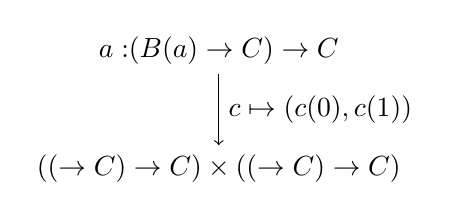
\begin{tikzpicture}
\node (N0) at (0,12) {$\prd{a:\Bool} (B(a) \to C) \to C$};
\node (N1) at (0,10.5) {$((\zero \to C) \to C) \times ((\one \to C) \to C)$};
\draw[->] (N0) -- node[right]{$c \mapsto (c(0), c(1))$} (N1);
\end{tikzpicture}
\end{center}
The type $\zero \to C$ is contractible with center $(\lambda b:\zero) \abort(C,b)$. We thus have an equivalence
\begin{center}
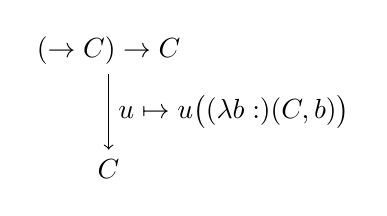
\begin{tikzpicture}
\node (N0) at (0,12) {$(\zero \to C) \to C$};
\node (N1) at (0,10.5) {$C$};
\draw[->] (N0) -- node[right]{$u \mapsto u\big((\lambda b:\zero) \abort(C,b)\big)$} (N1);
\end{tikzpicture}
\end{center}
Since the map $x \mapsto (\lambda \_:\one)x$ is an equivalence from $C$ to $\one \to C$, we have an equivalence
\begin{center}
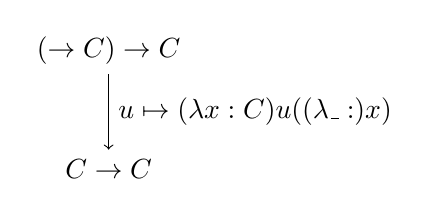
\begin{tikzpicture}
\node (N0) at (0,12) {$(\one \to C) \to C$};
\node (N1) at (0,10.5) {$C \to C$};
\draw[->] (N0) -- node[right]{$u \mapsto (\lambda x:C) u((\lambda \_:\one)x)$} (N1);
\end{tikzpicture}
\end{center}
Putting this all together, we see that the map 
\[ (C,c) \mapsto \Big(C,c\big(0,(\lambda b:\zero) \abort(C,b)\big),(\lambda x:C) c(1, (\lambda \_:\one)x)\Big)\] 
is an equivalence from $\WAlg(A,B)$ to $\NatAlg$.
\end{proof}

\begin{lemma}
For any $P$-algebra $\X : \WAlg(A,B)$ there is an equivalence
\[ \WFibAlgToNatFibAlg : \WFibAlg \; \X \to \NatFibAlg \; (\WAlgToNatAlg(\X)) \]
\end{lemma}
\begin{proof}
Let $(C,c)$ be a $P$-algebra and fix $E : C \to \U$. We have an equivalence
\begin{center}
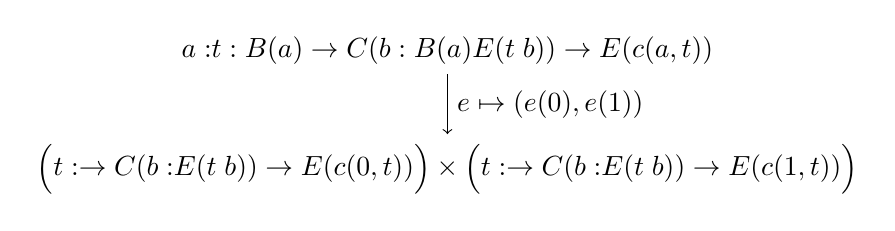
\begin{tikzpicture}
\node (N0) at (0,12) {$\prd{a:\Bool}\prd{t:B(a)\to C} (\prd{b:B(a)} E(t\;b)) \to E(c(a,t))$};
\node (N1) at (0,10.5) {$\Big(\prd{t:\zero\to C} (\prd{b:\zero} E(t\;b)) \to E(c(0,t))\Big) \times \Big(\prd{t:\one\to C} (\prd{b:\one} E(t\;b)) \to E(c(1,t))\Big)$};
\draw[->] (N0) -- node[right]{$e \mapsto (e(0), e(1))$} (N1);
\end{tikzpicture}
\end{center}
The type $\zero \to C$ is contractible with center $(\lambda b:\zero) \abort(C,b)$. Likewise, the type $\prd{b:\zero} E(\abort(C,b))$ is contractible with center 
$(\lambda b:\zero) \abort\big(E(\abort(C,b)),b\big)$. We thus have equivalences
\begin{center}
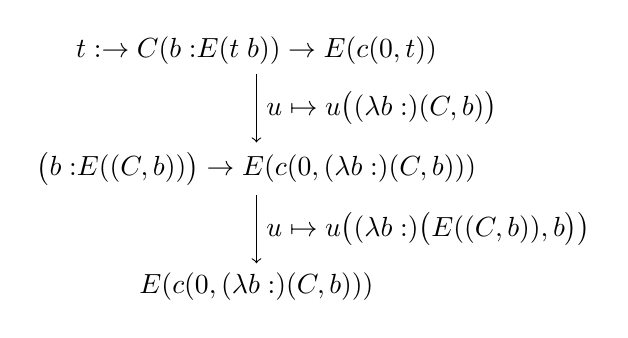
\begin{tikzpicture}
\node (N0) at (0,12) {$\prd{t:\zero\to C} (\prd{b:\zero} E(t\;b)) \to E(c(0,t))$};
\node (N1) at (0,10.5) {$\big(\prd{b:\zero} E(\abort(C,b))\big) \to E(c(0,(\lambda b:\zero) \abort(C,b)))$};
\node (N2) at (0,9) {$E(c(0,(\lambda b:\zero) \abort(C,b)))$};
\draw[->] (N0) -- node[right]{$u \mapsto u\big((\lambda b:\zero) \abort(C,b)\big)$} (N1);
\draw[->] (N1) -- node[right]{$u \mapsto u\big((\lambda b:\zero) \abort\big(E(\abort(C,b)),b\big)\big)$} (N2);
\end{tikzpicture}
\end{center}
The map $x \mapsto (\lambda \_:\one)x$ is an equivalence from $C$ to $\one \to C$. Likewise, for any $x:C$ the map $y \mapsto (\lambda \_:\one)y$  is an equivalence from $E(x)$ to $\one \to E(x)$. Thus, we have equivalences
\begin{center}
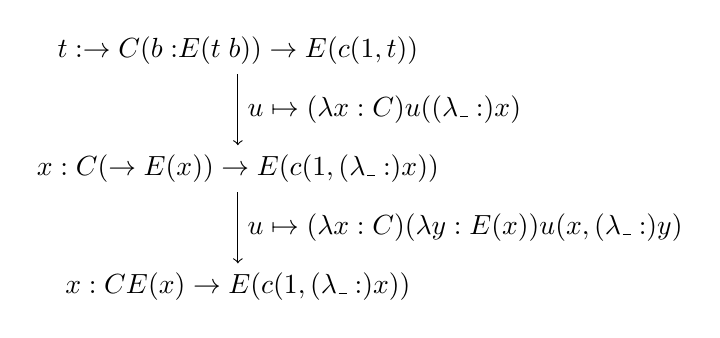
\begin{tikzpicture}
\node (N0) at (0,12) {$\prd{t:\one\to C} (\prd{b:\one} E(t\;b)) \to E(c(1,t))$};
\node (N1) at (0,10.5) {$\prd{x:C} (\one \to E(x)) \to E(c(1,(\lambda \_:\one)x))$};
\node (N2) at (0,9) {$\prd{x:C} E(x) \to E(c(1,(\lambda \_:\one)x))$};
\draw[->] (N0) -- node[right]{$u \mapsto (\lambda x:C) u((\lambda \_:\one)x)$} (N1);
\draw[->] (N1) -- node[right]{$u \mapsto (\lambda x:C) (\lambda y:E(x)) u(x,(\lambda \_:\one)y)$} (N2);
\end{tikzpicture}
\end{center}
Putting this all together, we see that the map 
\begin{align*}
& (E,e) \mapsto \Big(E,e\big(0,(\lambda b:\zero) \abort(C,b), (\lambda b:\zero) \abort\big(E(\abort(C,b)),b\big)\big),\\ & \;\;\;\;\;\;\;\;\;\;\;\;\;\;\;\;\;\;\;\;\;\;\;\; (\lambda x:C) (\lambda y:E(x)) e(1, (\lambda \_:\one)x), (\lambda \_:\one)y\Big)
\end{align*}
is an equivalence from $\WFibAlg \; (C,c)$ to $\NatFibAlg \; (\WAlgToNatAlg \; (C,c))$.
\end{proof}

\begin{lemma}
For any $P$-algebra $\X : \WAlg(A,B)$ and fibered $P$-algebra $\Y : \WFibAlg \; \X$ over $\X$ we have
\[ \WFibHom \; \Y \;\; \simeq \;\; \NatFibHom \; \big(\WFibAlgToNatFibAlg(\Y)\big) \]
\end{lemma}
\begin{proof}
Let $(C,c)$ be a $P$-algebra and $(E,e)$ be a fibered $P$-algebra over $(C,c)$. Fix a function $f : (\Pi x:C) E(x)$. We have an equivalence
\begin{center}
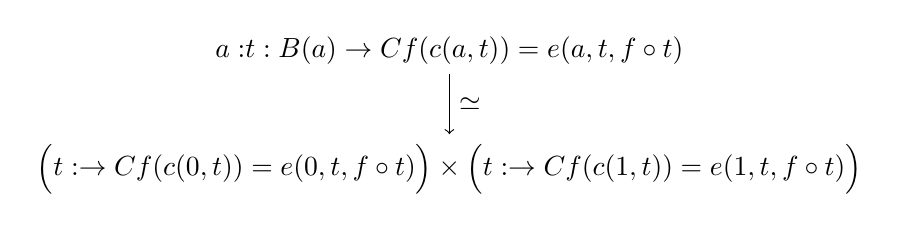
\begin{tikzpicture}
\node (N0) at (0,12) {$\prd{a:\Bool}\prd{t:B(a)\to C} f(c(a,t)) = e(a,t,f \circ t)$};
\node (N1) at (0,10.5) {$\Big(\prd{t:\zero\to C} f(c(0,t)) = e(0,t,f \circ t)\Big) \times \Big(\prd{t:\one\to C} f(c(1,t)) = e(1,t,f \circ t)\Big)$};
\draw[->] (N0) -- node[right]{$\simeq$} (N1);
\end{tikzpicture}
\end{center}
The type $\zero \to C$ is contractible with center $(\lambda b:\zero) \abort(C,b)$. Furthermore, since all functions out of $\zero$ having the same codomain are equal, we have
\[f \circ (\lambda b:\zero) \abort(C,b) = (\lambda b:\zero) \abort(E(\abort(C,b)), b)\]
This implies the following equivalences:
\begin{center}
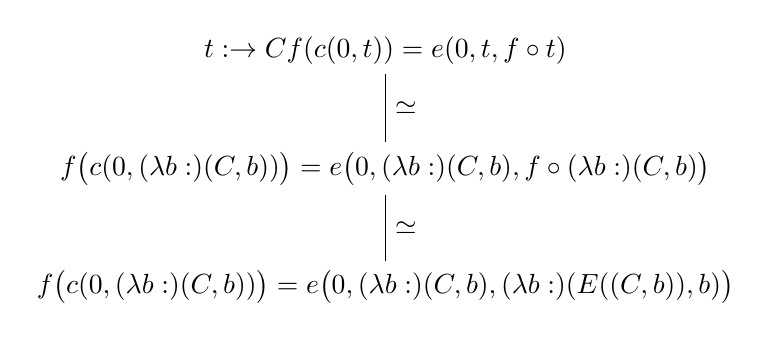
\begin{tikzpicture}
\node (N0) at (0,12) {$\prd{t:\zero\to C} f(c(0,t)) = e(0,t,f \circ t)$};
\node (N1) at (0,10.5) {$f\big(c(0,(\lambda b:\zero) \abort(C,b))\big) = e\big(0,(\lambda b:\zero) \abort(C,b), f \circ (\lambda b:\zero) \abort(C,b)\big)$};
\node (N2) at (0,9) {$f\big(c(0,(\lambda b:\zero) \abort(C,b))\big) = e\big(0,(\lambda b:\zero) \abort(C,b),(\lambda b:\zero) \abort(E(\abort(C,b)), b)\big)$};
\draw[-] (N0) -- node[right]{$\simeq$} (N1);
\draw[-] (N1) -- node[right]{$\simeq$} (N2);
\end{tikzpicture}
\end{center}
The map $x \mapsto (\lambda \_:\one)x$ is an equivalence from $C$ to $\one \to C$.  Thus, we have an equivalence
\begin{center}
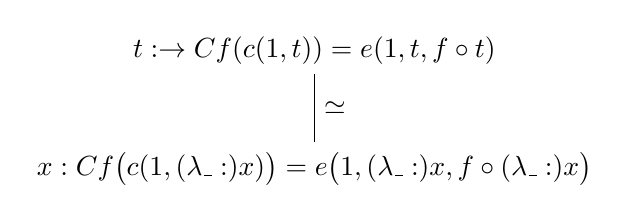
\begin{tikzpicture}
\node (N0) at (0,12) {$\prd{t:\one\to C} f(c(1,t)) = e(1,t,f \circ t)$};
\node (N1) at (0,10.5) {$\prd{x:C} f\big(c(1,(\lambda \_:\one)x)\big) = e\big(1,(\lambda \_:\one)x, f \circ (\lambda \_:\one)x\big)$};
\draw[-] (N0) -- node[right]{$\simeq$} (N1);
\end{tikzpicture}
\end{center}
This finishes the proof.
\end{proof}

\begin{corollary}
For any $P$-algebras $\X,\Y : \WAlg(A,B)$ we have
\[ \WHom \; \X \; \Y \;\; \simeq \;\; \NatHom \; \big(\WAlgToNatAlg(\X)\big) \; \big(\WAlgToNatAlg(\Y)\big) \]
\end{corollary}

\begin{corollary}
For any $\nat$-algebra $\X : \NatAlg$ we have
\begin{alignat*}{4}
& \IsNatHInit(\X) \;\; & \simeq \;\; & \IsWHInit(\WAlgToNatAlg^{-1}(\X)) \\
& \IsNatHProj(\X) \;\; & \simeq \;\; & \IsWHProj(\WAlgToNatAlg^{-1}(\X))
\end{alignat*}
\end{corollary}

\begin{theorem}\label{lem:WMainInternal}
For a $\nat$-algebra $\X : \NatAlg$, we have
\[ \IsNatHProj \; \X \;\;\; \leftrightarrow \;\;\; \IsNatHInit \; \X \]
Moreover, both types are mere propositions; hence in particular we have
\[ \IsNatHProj \; \X \;\;\; \simeq \;\;\; \IsNatHInit \; \X \]
\end{theorem}

\begin{corollary}\label{lem:NatInitInt}
The $\nat$ algebra $(\nat,\z,\suc(-)) : \NatAlg$ is homotopy-initial.
\end{corollary}

